\section{BVR FUNDAMENTALS}
\label{subsec:bvr}

\subsection[AR FUNDAMENTALS]{ACTIVE RADAR MISSILE FUNDAMENTALS}

\begin{figure}[htbp]
    \centering
    \begin{tikzpicture}[figstyle]
        % help lines
        % \draw[help lines] (0,-10) grid (100,10);

        % MISSILE
        \coordinate (A_missile) at (0,0);
        \coordinate (B_missile) at (30,10);
        \coordinate (C_missile) at (60,3);
        \coordinate (D_missile) at (80,0);

        \draw[thick, ->]
        (A_missile) .. controls ($(A_missile)+(20,0)$) and ($(B_missile)+(-10,0)$) .. 
        (B_missile) .. controls ($(B_missile)+(5,0)$) and ($(C_missile)+(-10,2.5)$) ..
        (C_missile);
        \draw[dotted, thick, ->] 
        (C_missile) .. controls ($(C_missile)+(10,-2.5)$) and ($(D_missile)+(-5,0)$) ..
        (D_missile);

        \node[above] at (A_missile) {\titlefont A};
        \node[above] at (B_missile) {\titlefont B};
        \node[above] at (C_missile) {\titlefont C};
        \node[above] at (D_missile) {\titlefont D};

        % FIGHTER
        \coordinate (A_fighter) at (A_missile);
        \coordinate (C_fighter) at ($(A_fighter)+(20,0)$);
        \coordinate (D_fighter) at ($(C_fighter)+(-5,-5)$);

        \node[
            anchor=east,
        ] (fig_A_fighter) at (A_fighter) {
            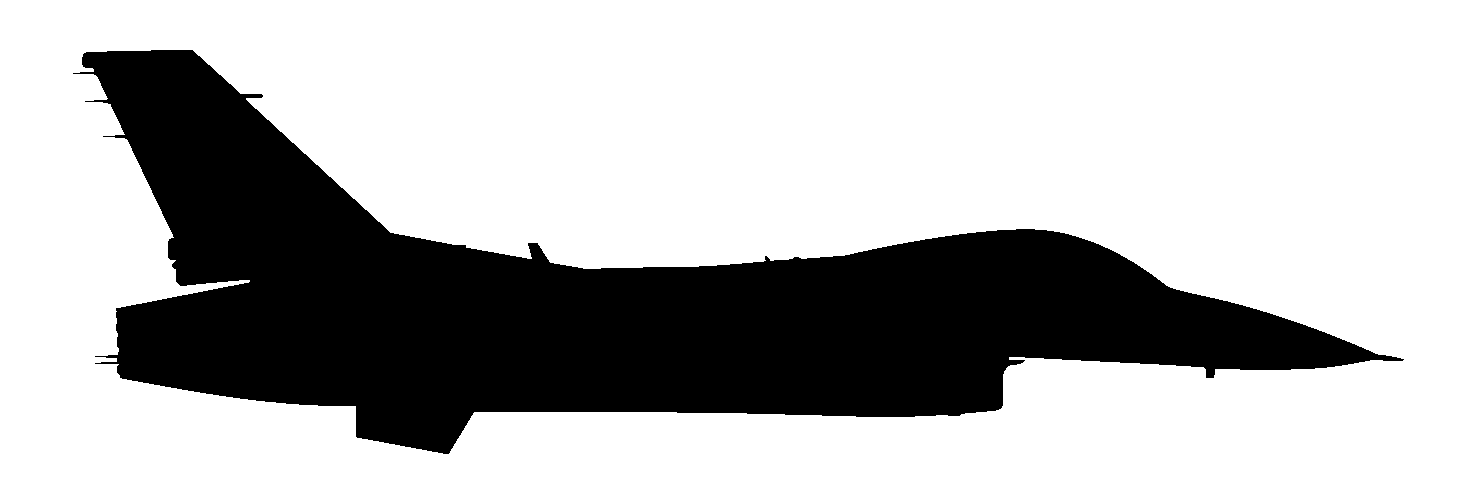
\includegraphics[
                width=7.5mm,
            ]{diagrams/aircraft/silhouette_f16_side.pdf}
        };

        \draw[ultra thick, ->] 
        (A_fighter) -- 
        (C_fighter) .. controls ($(C_fighter)+(5,0)$) and ($(C_fighter)+(5,-5)$) .. 
        ($(C_fighter)+(0,-5)$) --
        (D_fighter);

        \node[above right] at (C_fighter) {\titlefont C};
        \node[left] at (D_fighter) {\titlefont D};

        % BANDIT
        \coordinate (A_bandit) at (100,0);
        \coordinate (C_bandit) at (85,0);
        \coordinate (D_bandit) at (D_missile);

        \draw[ultra thick, ->] 
        (A_bandit) -- 
        (D_bandit);

        \node[above] at (A_bandit) {\titlefont A};
        \node[above] at (C_bandit) {\titlefont C};

        \filldraw[red] (D_bandit) circle (2pt);

        % Distance lines
        \draw[thin, <->]
        ($(C_fighter)+(0,-12.5)$) -- node[pos=0.5, above]{\small\titlefont R\textsubscript{A-POLE}}
        ($(C_bandit)+(0,-12.5)$);
        \draw[thin, <->]
        (15,-20) -- node[pos=0.5, above]{\small\titlefont R\textsubscript{F-POLE}}
        ($(D_missile)+(0,-20)$);
        \draw[thin, <->]
        ($(A_missile)+(0,-27.5)$) -- node[pos=0.5, above]{\small\titlefont R\textsubscript{LAUNCH}}
        ($(A_bandit)+(0,-27.5)$);

        \draw[thin]
        ($(C_fighter)+(0,-2.5)$) -- ($(C_fighter)+(0,-15)$)
        ($(C_bandit)+(0,-2.5)$) -- ($(C_bandit)+(0,-15)$)
        ($(D_fighter)+(0,-2.5)$) -- (15,-22.5)
        ($(D_missile)+(0,-2.5)$) -- ($(D_missile)+(0,-22.5)$)
        ($(A_missile)+(0,-2.5)$) -- ($(A_missile)+(0,-30)$)
        ($(A_bandit)+(0,-2.5)$) -- ($(A_bandit)+(0,-30)$);

    \end{tikzpicture}
    \caption{Side-on view of a generic AIM-120 employment profile}
    \label{fig:aa_weap:bvr:aim120profile}
    % TODO: silhouettes?
\end{figure}

\begin{tcoloritemize}
    \blueitem[AIM-120 \break Employment \break Profile]
    \Cref{fig:aa_weap:bvr:aim120profile} shows the trajectories of fighter, bandit \& missile for a generic AIM-120 employment profile
    including the following phases

    \begin{itemize}
        \item \textbf{A --- Launch / Boost Phase}
        \item \textbf{B --- Mid-Course Phase}
        \item \textbf{C --- Acquisition}
        \item \textbf{D --- Intercept}
    \end{itemize}
    \blueitem[Launch / Boost Phase]
    \textbf{Boost}

    \begin{itemize}
        \item Motor only fires for initial seconds of flight 
        \item After burnout missile \textbf{\underline{cannot gain energy}}
    \end{itemize}

    \textbf{Lofting} 

    \begin{itemize}
        \item To reach longer ranges missile ``lofts'' itself to conserve energy \& optimize trajectory
        \item Pilot can manually loft by raising the nose 20-30 deg prior to launch
    \end{itemize}
    \blueitem[Mid-Course Phase]
    \textbf{Missile flies using internal IMU}

    \begin{itemize}
        \item Receives periodic datalink updates
        \item Will fly to last updated target position if DL lost
    \end{itemize}
    \blueitem[Acquisition \& MPRF ``Active'' Phase]
    \textbf{Missile radar turns on once close to target location}
    \begin{itemize}
        \item Seeker in MPRF (Medium Pulse Repetition Frequency) mode 
        \item Locks on to closest / best target
    \end{itemize}
    \blueitem[Terminal Phase \& Intercept]
    \textbf{Once missile seeker has acquired target}
    \begin{itemize}
        \item Flies PNG intercept trajectory
        \item Requires no further DL support, fighter can turn away from the bandit
    \end{itemize}
\end{tcoloritemize}

\cautionbox{
    \textbf{Do NOT employ AIM-120 without clear avenue-of-fire} 
    \begin{itemize}
        \item AIM-120 has NO IFF functionality
    \end{itemize}
}

\subsubsection{TACTICAL CONSIDERATIONS}
\label{subsec:bvr:tacticalconsideration}
% \label{subsec:aim120:tactics}
\begin{tcoloritemize}
    \blueitem[Range Definitions]
    \textbf{Fighter-bandit distance} can be measured at different points during the timeline

    \begin{itemize}
        \item \textbf{R\textsubscript{Launch}} --- distance at launch
        \item \textbf{R\textsubscript{A-Pole}} --- distance when missile goes active
        \item \textbf{R\textsubscript{F-Pole}} --- distance at impact
    \end{itemize}
    
    These are also illustrated in \cref{fig:aa_weap:bvr:aim120profile}.
    \blueitem[Maximizing Launch Range / Energy]
    \textbf{Why?}
    \begin{itemize}
        \item Ability to launch at longer ranges forces bandit defensive
        \item Bandit may not be able to counter-launch
        \item Higher launch energy increases P\textsubscript{intercept} %probability of intercept
    \end{itemize}
    \textbf{How?}
    \begin{itemize}
        \item \textbf{High velocity} --- increases kinetic energy 
        \item \textbf{High altitude} --- increases potential energy, reduces drag
    \end{itemize}
    \blueitem[Maximizing \break F-Pole Range]
    \textbf{Why?}
    \begin{itemize}
        \item Less likely to enter bandit launch envelope
        \item More time/range to launch 2nd missile if necessary
    \end{itemize}
    \textbf{How?}
    \begin{itemize}
        \item \textbf{Crank} --- turn 45-60 degrees away from bandit to reduce closure rate, maintain radar contact
        \item \textbf{Dive} --- reduces threat missile envelope
    \end{itemize}
    \blueitem[Flowing Cold]
    \textbf{Why?}
    \begin{itemize}
        \item Missile requires no support once active
        \item Defend against unknown missile launches
        \item Maximize F-pole range further
    \end{itemize}
    \textbf{How?}
    \begin{itemize}
        \item \textbf{Turn} --- Away from bandit / threat
        \item \textbf{Dive} --- if necessary, reduces threat missile envelope 
    \end{itemize}
    \blueitem[Effect of Bandit Maneuvers]
    As evident in \cref{fig:aa_weap:bvr:aim120profile}, 
   \textbf{R\textsubscript{Launch}} is significantly greater than the distance travelled by the missile
    \begin{itemize}
        \item \textbf{DLZ calculated based off \underline{both} fighter \underline{and} bandit velocity/altitude}
        \item Bandit can significantly change missile envelope by reducing closure rate / altitude
        \item Post-launch bandit maneuvers can result in missile not having energy to intercept
    \end{itemize}
\end{tcoloritemize}

\clearpage

\subsection{FIGHTER MANEUVERS}

\begin{tcoloritemize}
    \blueitem[Crank]
    Fighter turns \textbf{45-60 deg} away from threat 

    \begin{itemize}
        \item reduces closure while maintaining radar track
        \item typically used post-launch
    \end{itemize}
    
    Reference \cref{fig:aa_weap:bvr:fightermaneuver:crank}
    \blueitem[Notch]
    Fighter turns \textbf{70-110 deg} away from threat

    \begin{itemize}
        \item minimizes relative velocity to break hostile pulse-doppler radar track
        \item increases angular motion, forcing missile to maneuver and expend energy
    \end{itemize}
    
    Reference \cref{fig:aa_weap:bvr:fightermaneuver:notch}
    \blueitem[Go Cold]
    Fighter turns \textbf{away} from threat

    \begin{itemize}
        \item used to kinematically defeat threat missiles
    \end{itemize}
    
    Reference \cref{fig:aa_weap:bvr:fightermaneuver:cold}
\end{tcoloritemize}

\begin{figure}[htbp]
    \centering
    \begin{subfigure}[b]{0.3\linewidth}
        \centering
        \begin{tikzpicture}[figstyle]
            % FIGHTER
            \node[
                anchor=north,
                yshift=1mm,
            ] (fighter) at (0,0) {
                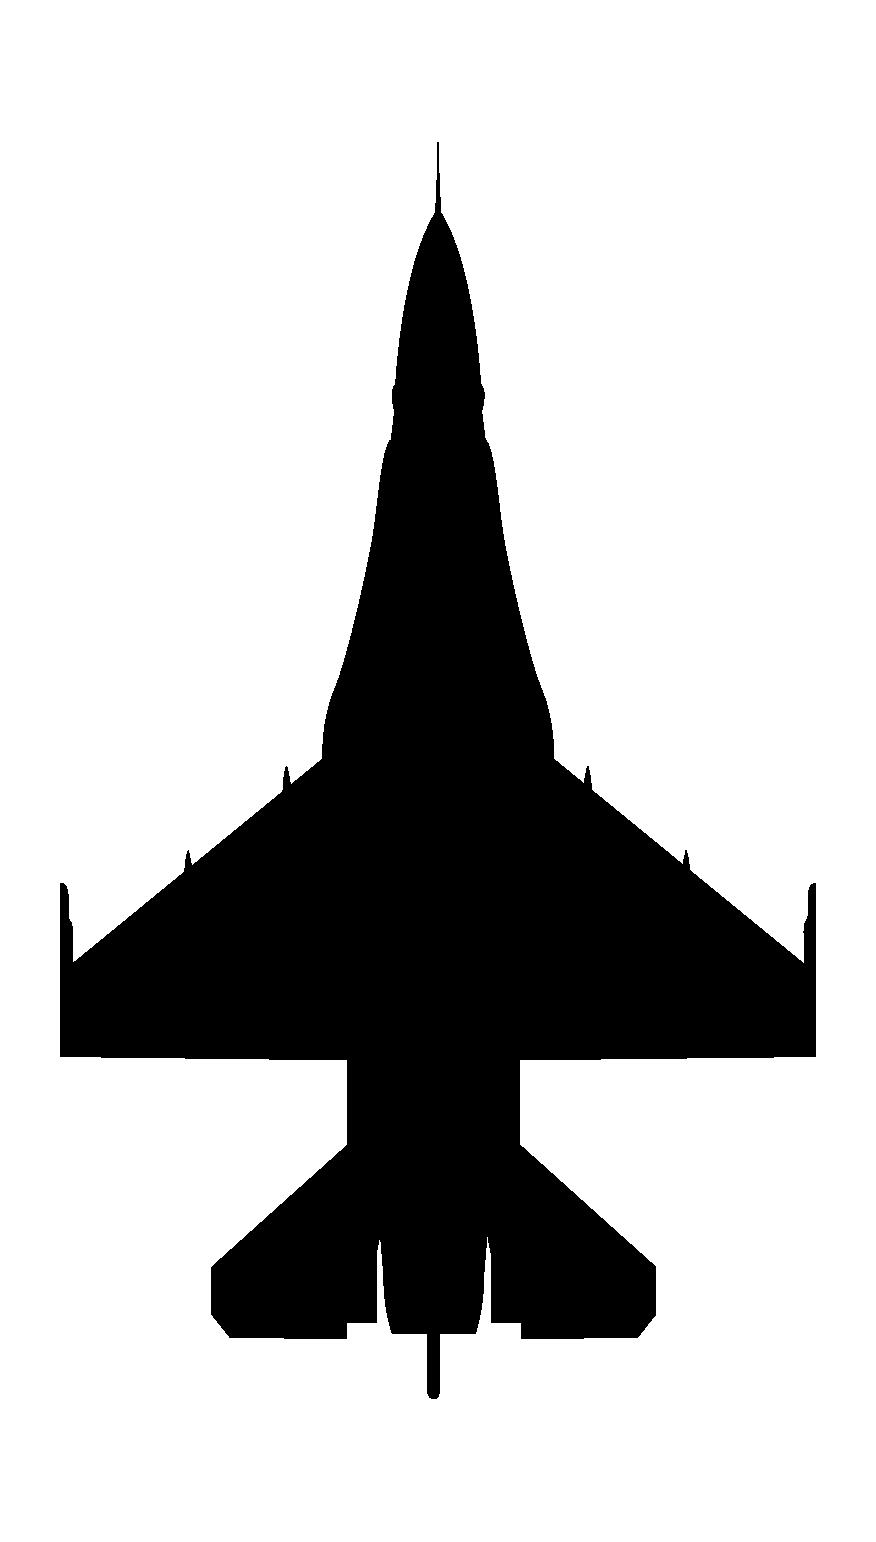
\includegraphics[
                    width=7.5mm,
                ]{diagrams/aircraft/silhouette_f16_top.pdf}
            };
            \draw[rounded corners, ->] 
            (0,0) -- (0,5) -- +(30:15) node[rotate=-60, anchor=south, yshift=-1mm]{
                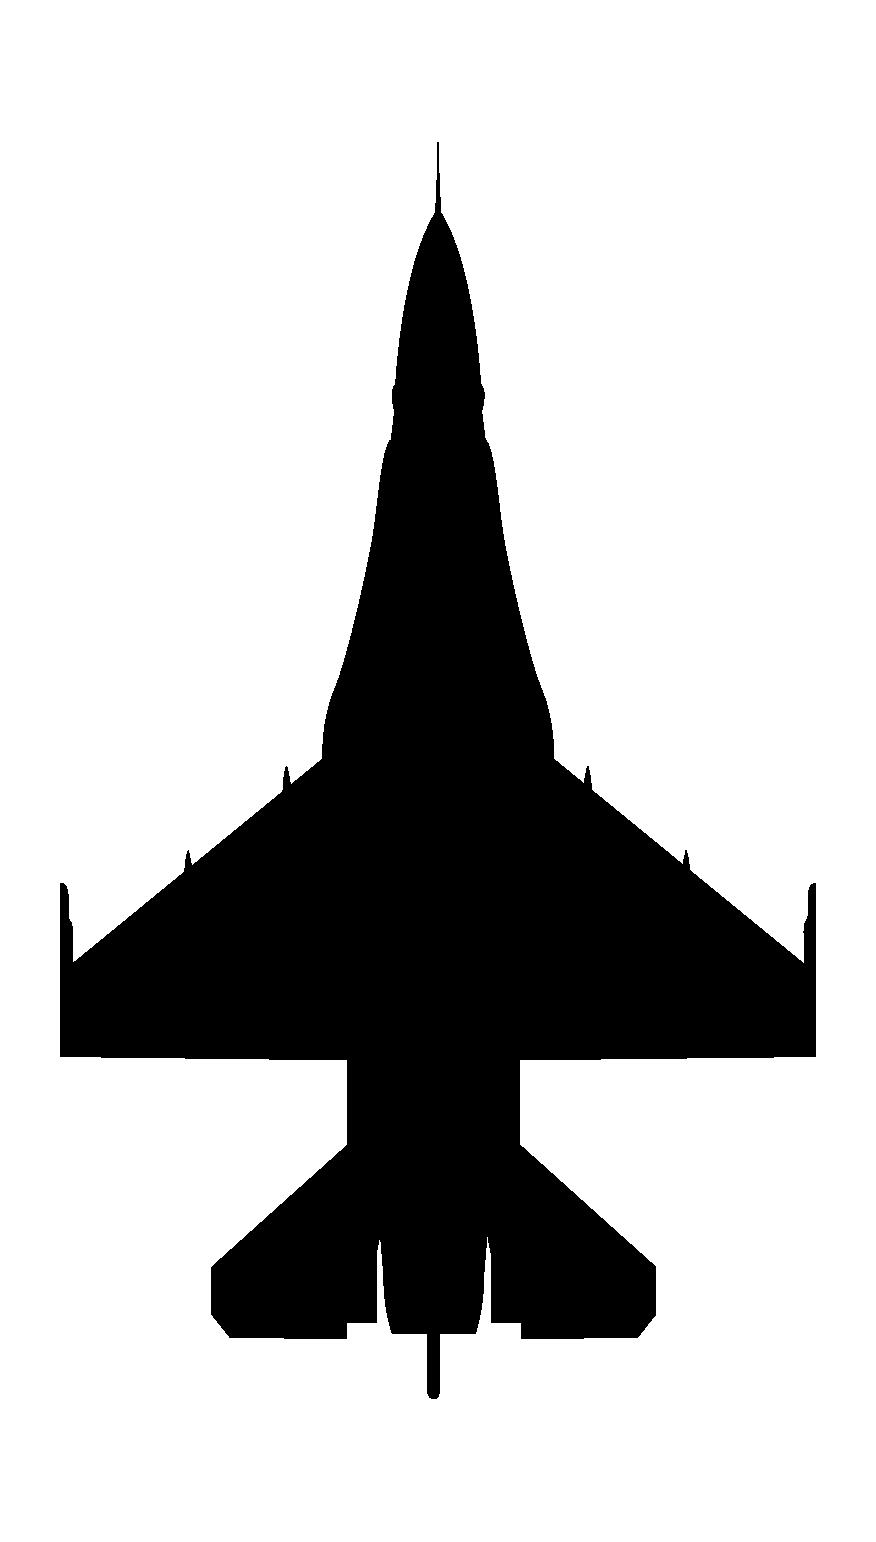
\includegraphics[
                width=7.5mm,
            ]{diagrams/aircraft/silhouette_f16_top.pdf}};
    
            % BANDIT
            \draw[rounded corners, ->] 
            (0,35) -- (0,25);
    
            % help line
            \draw[thin, dashed] 
            (0,25) -- (0,5);
    
            \draw[thin]
            (0,15) arc (90:30:10) node[pos=0.15, above right]{\small\titlefont 45-60$^\circ$};
    
        \end{tikzpicture}
        \caption{Crank}
        \label{fig:aa_weap:bvr:fightermaneuver:crank}
    \end{subfigure}
    \begin{subfigure}[b]{0.3\linewidth}
        \centering
        \begin{tikzpicture}[figstyle]
            % FIGHTER
            \node[
                anchor=north,
                yshift=1mm,
            ] (fighter) at (0,0) {
                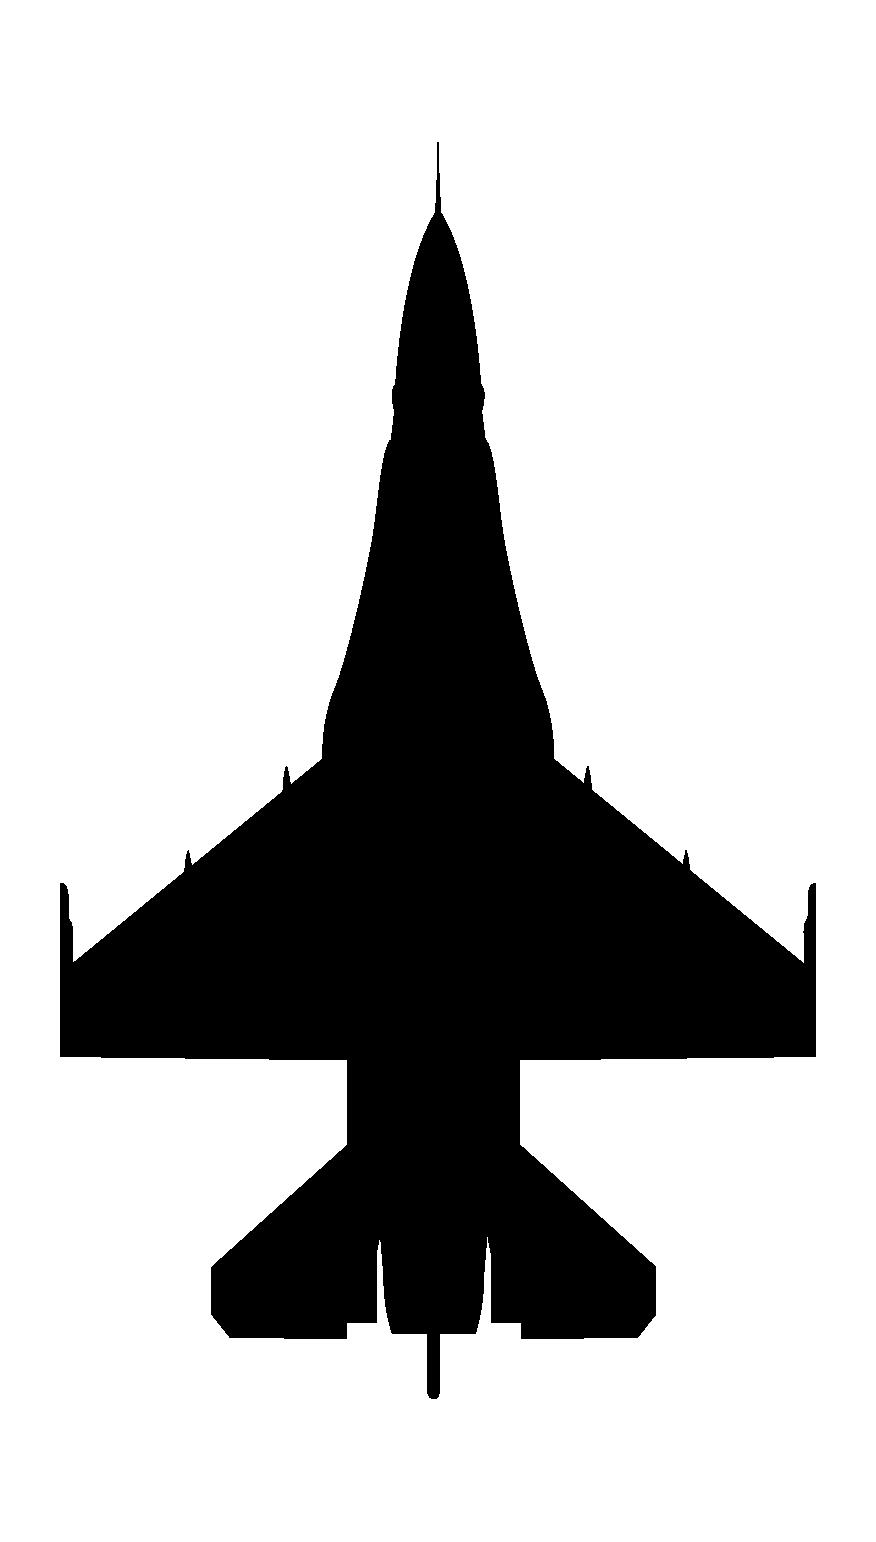
\includegraphics[
                    width=7.5mm,
                ]{diagrams/aircraft/silhouette_f16_top.pdf}
            };
            \draw[rounded corners, ->] 
            (0,0) -- (0,5) -- +(0:15) node[rotate=-90, anchor=south, yshift=-1mm]{
                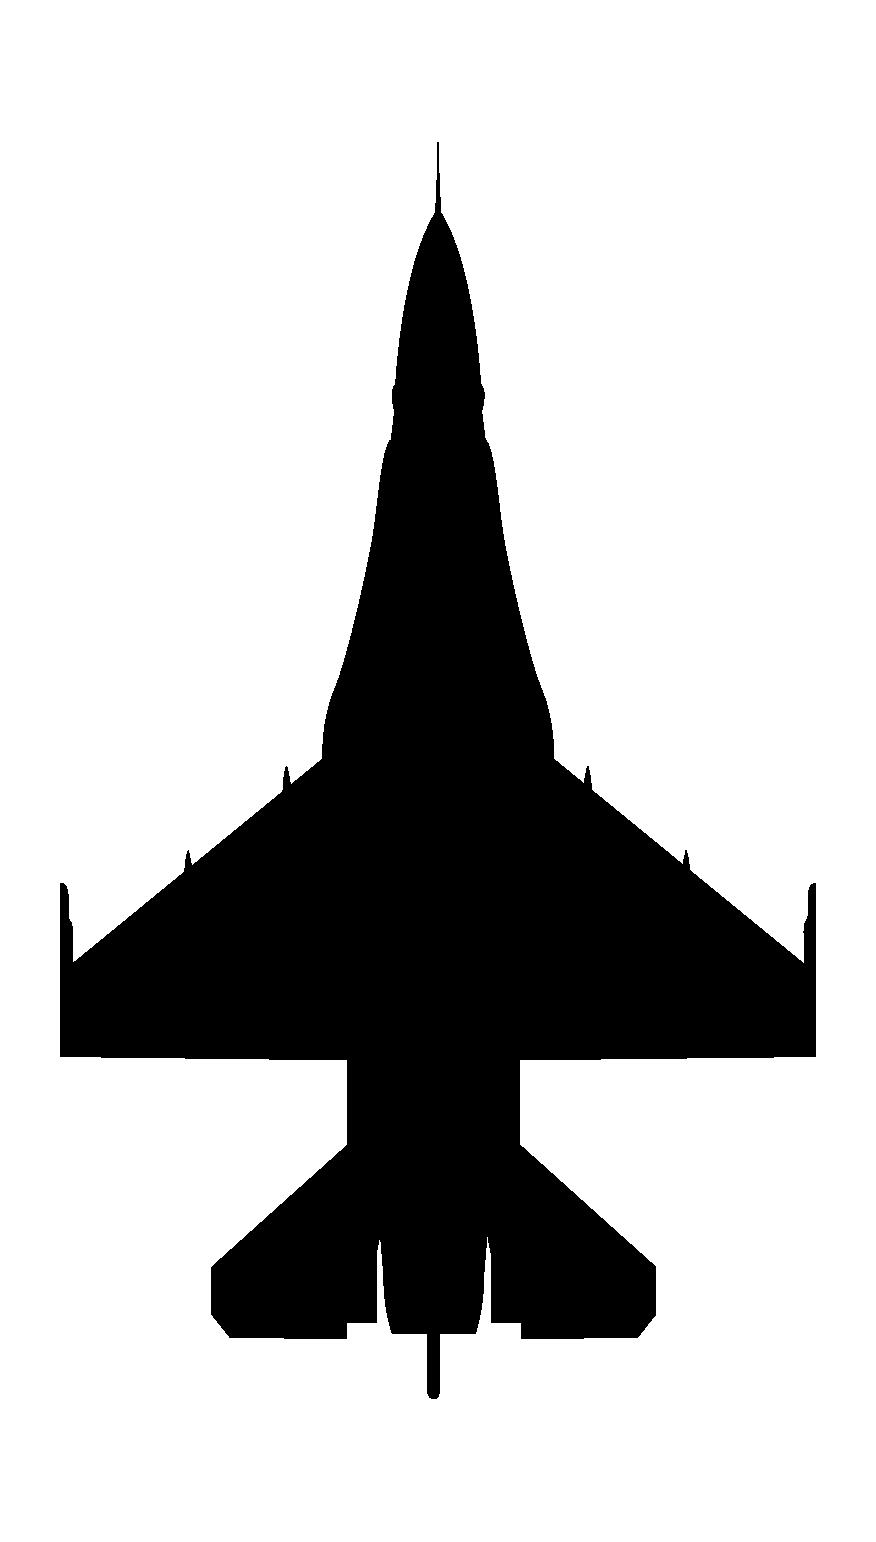
\includegraphics[
                width=7.5mm,
            ]{diagrams/aircraft/silhouette_f16_top.pdf}};
    
            % BANDIT
            \draw[rounded corners, ->] 
            (0,35) -- (0,25);
    
            % help line
            \draw[thin, dashed] 
            (0,25) -- (0,5);
    
            \draw[thin]
            (0,15) arc (90:0:10) node[pos=0.5, above right]{\small\titlefont 70-110$^\circ$};
    
        \end{tikzpicture}
        \caption{Notch}
        \label{fig:aa_weap:bvr:fightermaneuver:notch}
    \end{subfigure}
    \begin{subfigure}[b]{0.3\linewidth}
        \centering
        \begin{tikzpicture}[figstyle]
            % FIGHTER
            \node[
                anchor=north,
                yshift=1mm,
            ] (fighter) at (0,0) {
                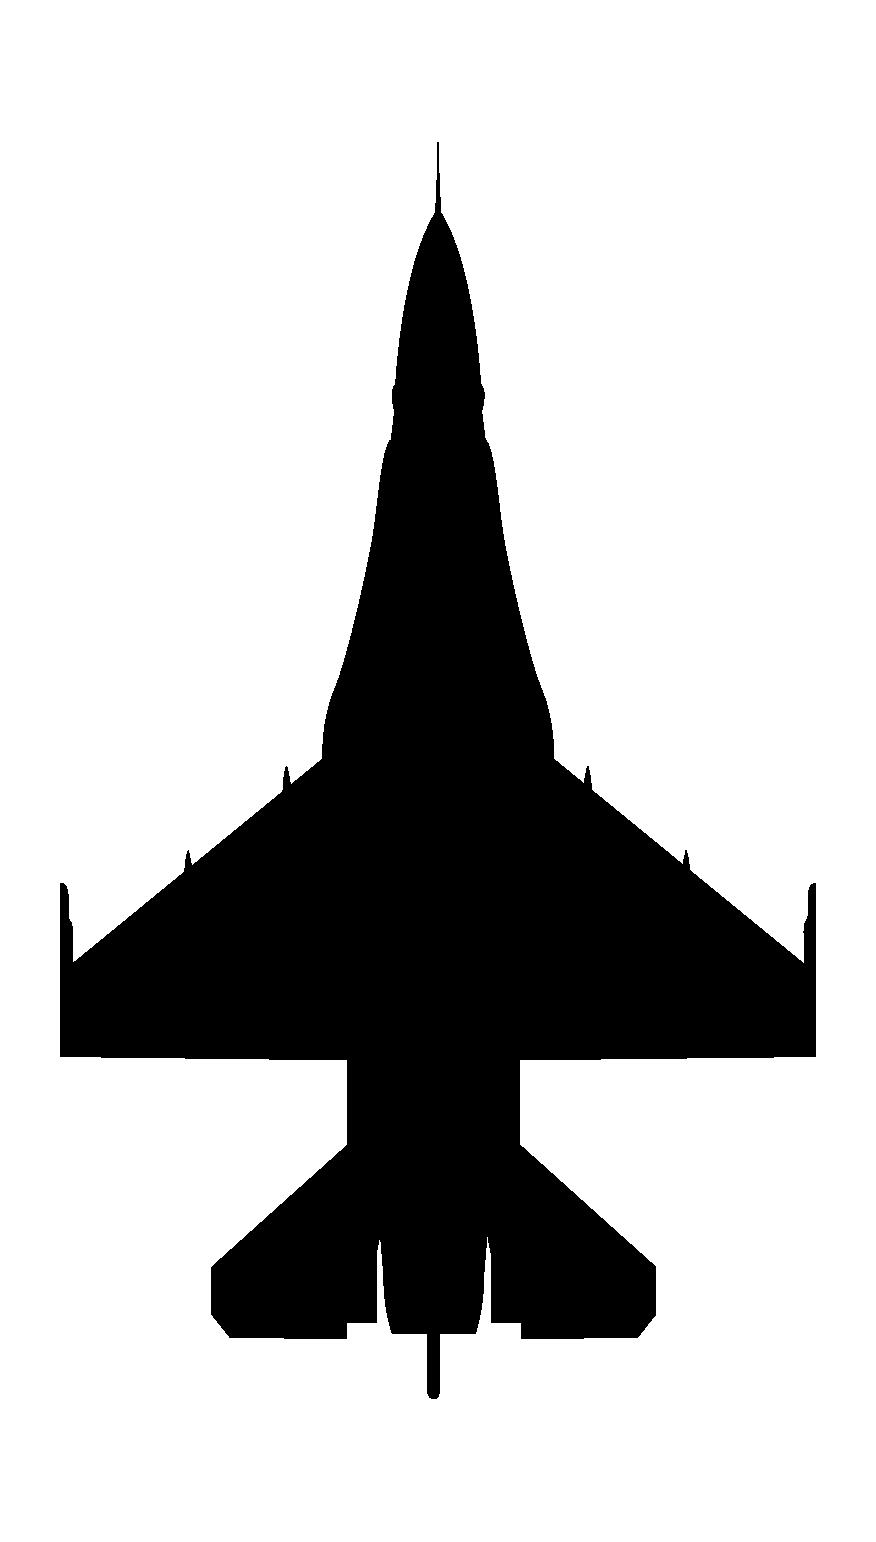
\includegraphics[
                    width=7.5mm,
                ]{diagrams/aircraft/silhouette_f16_top.pdf}
            };
            \draw[->] 
            (0,0) -- 
            (0,5) arc (180:0:5) --
            (10,0) 
            node[rotate=-180, anchor=south, yshift=-1mm]{
                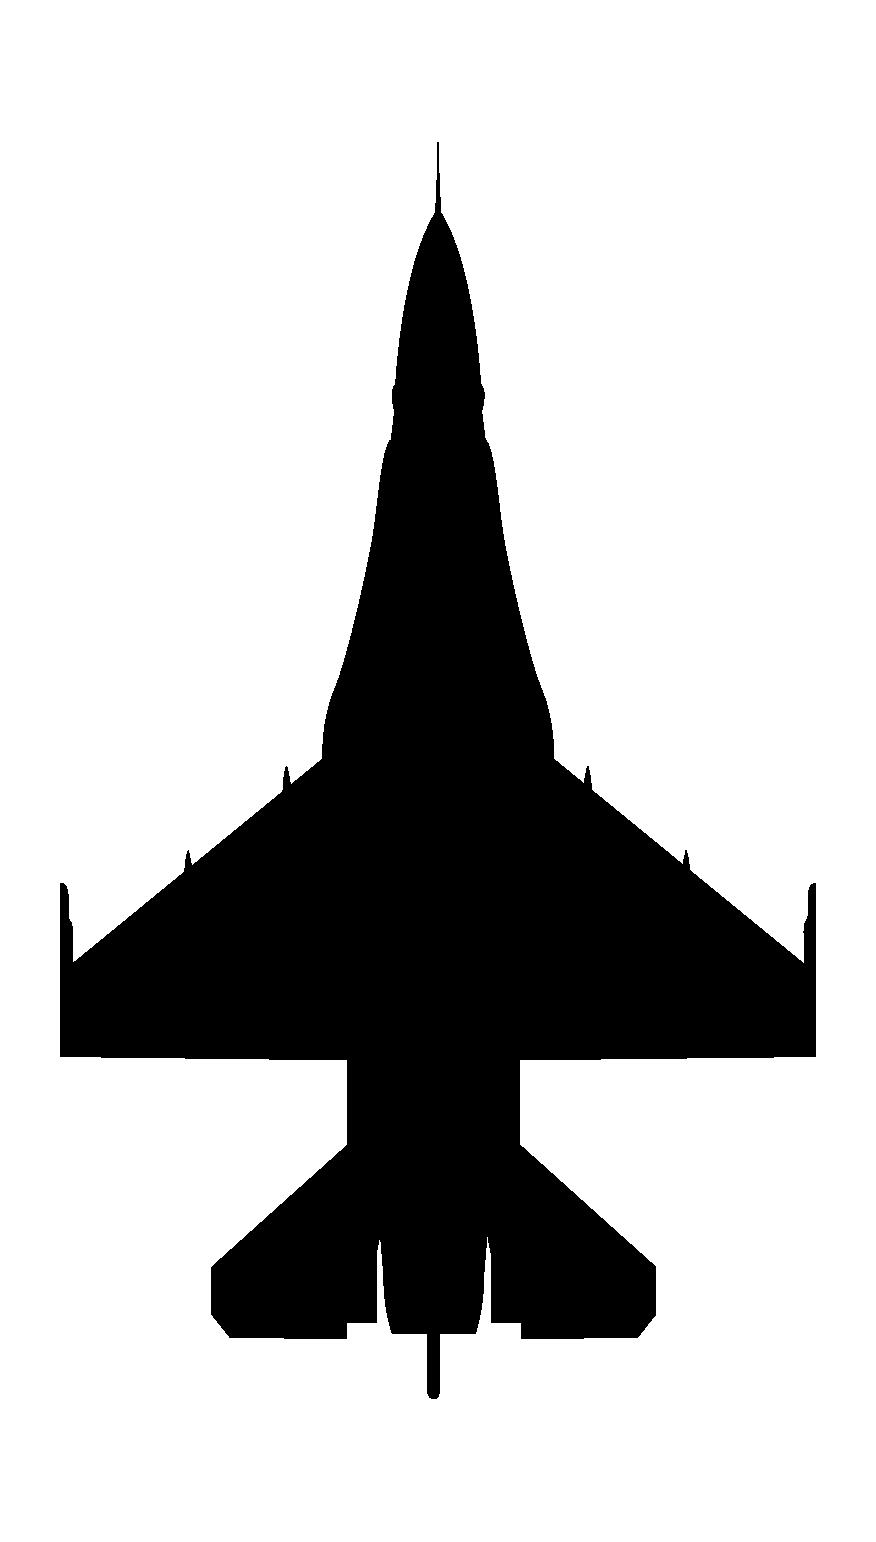
\includegraphics[
                width=7.5mm,
            ]{diagrams/aircraft/silhouette_f16_top.pdf}};
    
            % BANDIT
            \draw[rounded corners, ->] 
            (0,35) -- (0,25);

            % help line
            \draw[thin, dashed] 
            (0,25) -- (0,5);

        \end{tikzpicture}
        \caption{Go Cold}
        \label{fig:aa_weap:bvr:fightermaneuver:cold}
    \end{subfigure}
    \caption{Top-down view of basic BVR fighter maneuvers}
    \label{fig:aa_weap:bvr:fightermaneuver}
\end{figure}

\notebox{
    \textbf{Turning in after going cold can place fighter within bandit launch envelope}
}

\subsection{TARGET ASPECT}

\begin{tcoloritemize}
    \blueitem[Target Aspect]
    Angle between imaginary line connecting fighter-bandit and bandit heading
    \blueitem[Hot]
    \textbf{Target aspect --- 0-40 deg}
    \begin{itemize}
        \item offensive posture, maximizes closure
    \end{itemize}
    \blueitem[Flank]
    \textbf{Target aspect --- 40-70 deg}
    \begin{itemize}
        \item minimizes closure while maintaining radar track
    \end{itemize}
    \blueitem[Beam]
    \textbf{Target aspect --- 70-110 deg}
    \begin{itemize}
        \item defensive maneuver to break pulse-doppler radar track
    \end{itemize}
    \blueitem[Drag]
    \textbf{Target aspect --- 110-180 deg}
    \begin{itemize}
        \item defense to kinematically defeat missile
        \item often used in group tactics as ambush setup
    \end{itemize}
\end{tcoloritemize}

\begin{figure}[htbp]
    \centering
    \begin{subfigure}[b]{0.2\linewidth}
        \centering
        \begin{tikzpicture}[figstyle]
            % FIGHTER
            \node[
                anchor=north,
                yshift=1mm,
            ] (fighter) at (0,0) {
                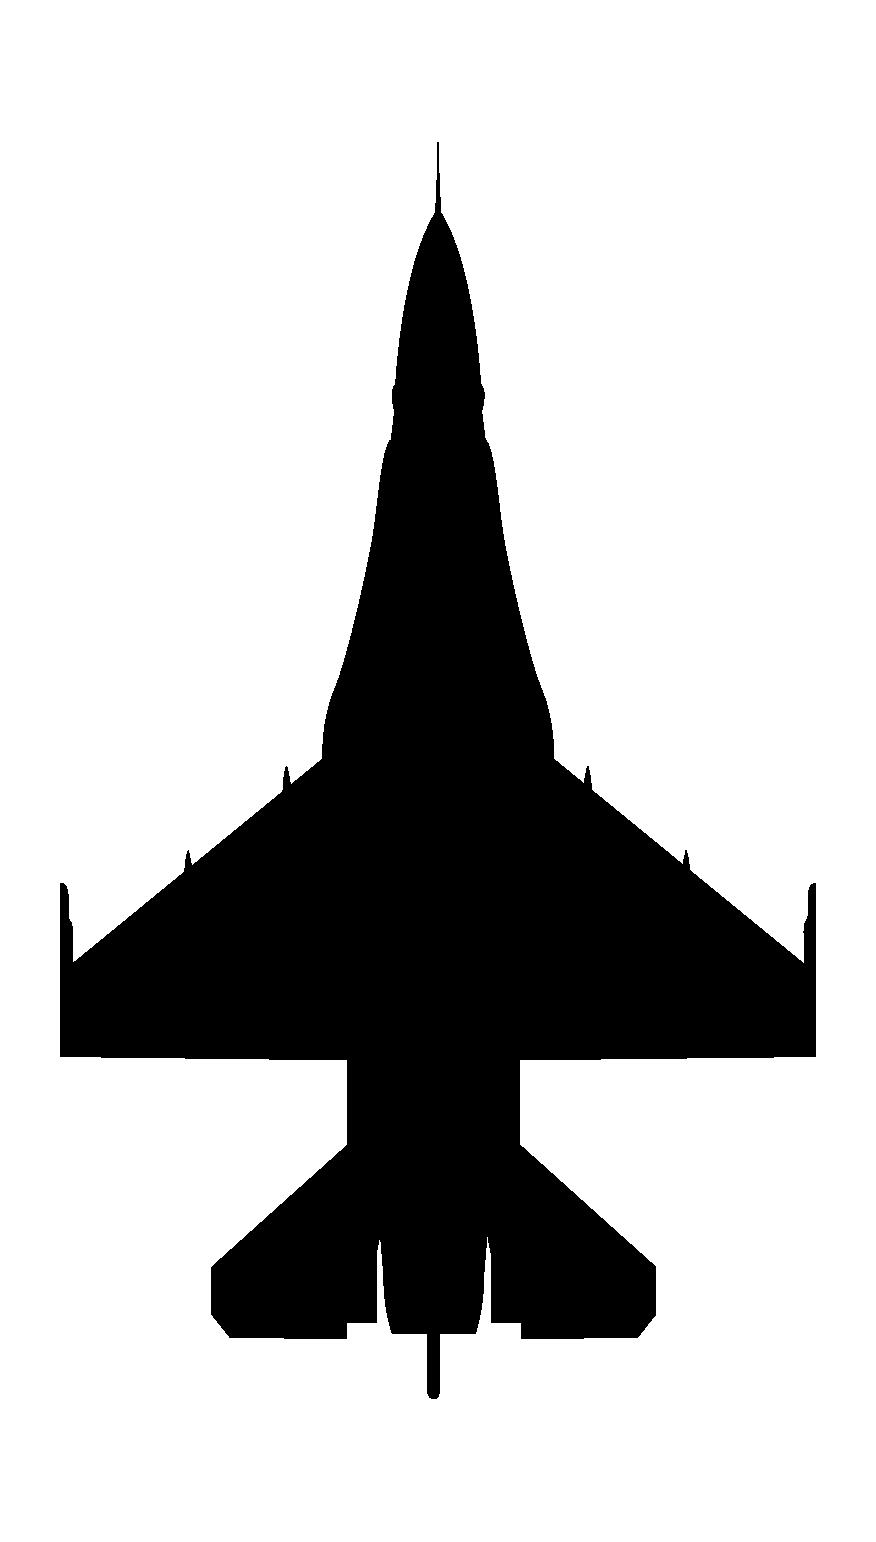
\includegraphics[
                    width=7.5mm,
                ]{diagrams/aircraft/silhouette_f16_top.pdf}
            };
    
            % BANDIT
            \draw[rounded corners, ->] 
            (0,20) -- +(-75:15);
    
            % help line
            \draw[thin, dashed] 
            (0,20) -- (0,0);
    
            \draw[thin]
            (0,10) arc (-90:-75:10) node[pos=1.0, right]{\small\titlefont 0-40$^\circ$};

        \end{tikzpicture}
        \caption{Hot}
        \label{fig:aa_weap:bvr:ta:hot}
    \end{subfigure}
    \begin{subfigure}[b]{0.2\linewidth}
        \centering
        \begin{tikzpicture}[figstyle]
            % FIGHTER
            \node[
                anchor=north,
                yshift=1mm,
            ] (fighter) at (0,0) {
                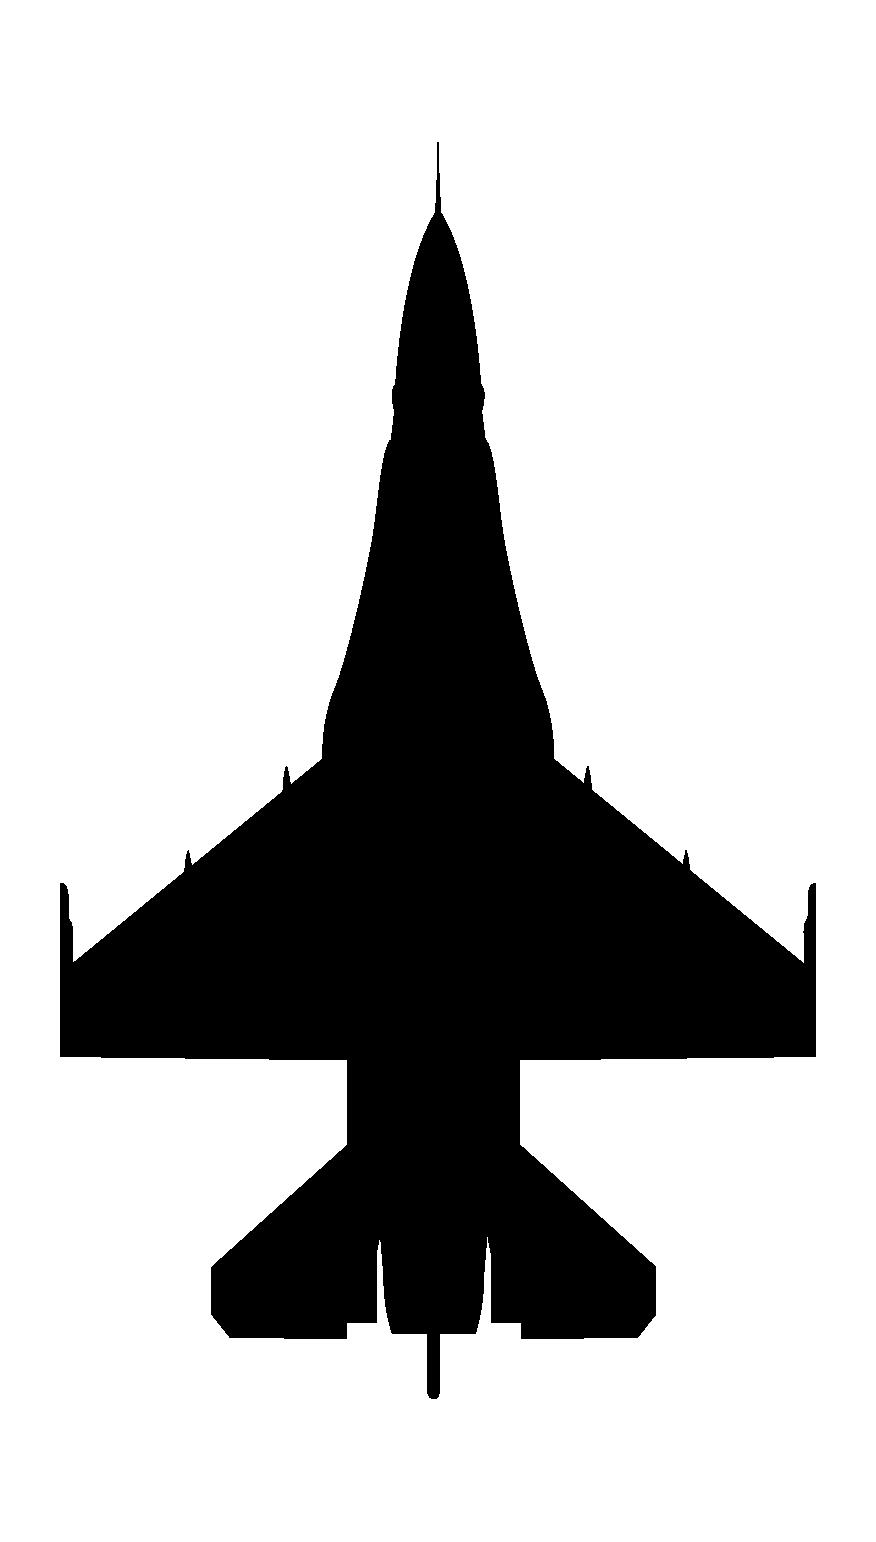
\includegraphics[
                    width=7.5mm,
                ]{diagrams/aircraft/silhouette_f16_top.pdf}
            };
    
            % BANDIT
            \draw[rounded corners, ->] 
            (0,20) -- +(-30:15);
    
            % help line
            \draw[thin, dashed] 
            (0,20) -- (0,0);
    
            \draw[thin]
            (0,10) arc (-90:-30:10) node[pos=0.25, below right]{\small\titlefont 40-70$^\circ$};

        \end{tikzpicture}
        \caption{Flank}
        \label{fig:aa_weap:bvr:ta:flank}
    \end{subfigure}
    \begin{subfigure}[b]{0.25\linewidth}
        \centering
        \begin{tikzpicture}[figstyle]
            % FIGHTER
            \node[
                anchor=north,
                yshift=1mm,
            ] (fighter) at (0,0) {
                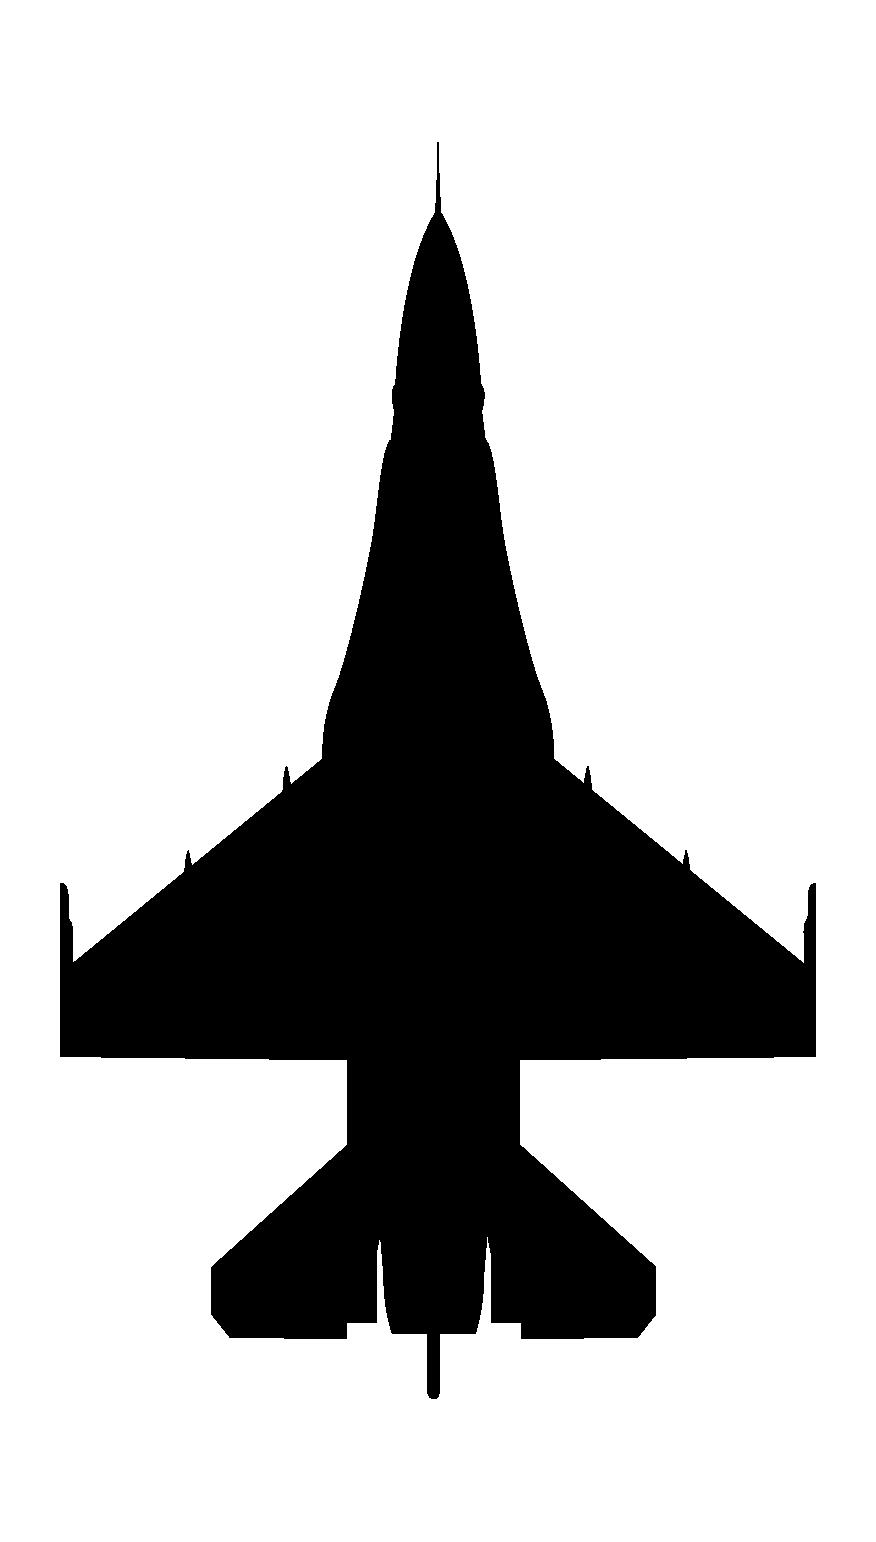
\includegraphics[
                    width=7.5mm,
                ]{diagrams/aircraft/silhouette_f16_top.pdf}
            };
    
            % BANDIT
            \draw[rounded corners, ->] 
            (0,20) -- +(0:15);
    
            % help line
            \draw[thin, dashed] 
            (0,20) -- (0,0);
    
            \draw[thin]
            (0,10) arc (-90:0:10) node[pos=0.25, below right]{\small\titlefont 70-110$^\circ$};
    
        \end{tikzpicture}
        \caption{Beam}
        \label{fig:aa_weap:bvr:ta:beam}
    \end{subfigure}
    \begin{subfigure}[b]{0.25\linewidth}
        \centering
        \begin{tikzpicture}[figstyle]
            % FIGHTER
            \node[
                anchor=north,
                yshift=1mm,
            ] (fighter) at (0,0) {
                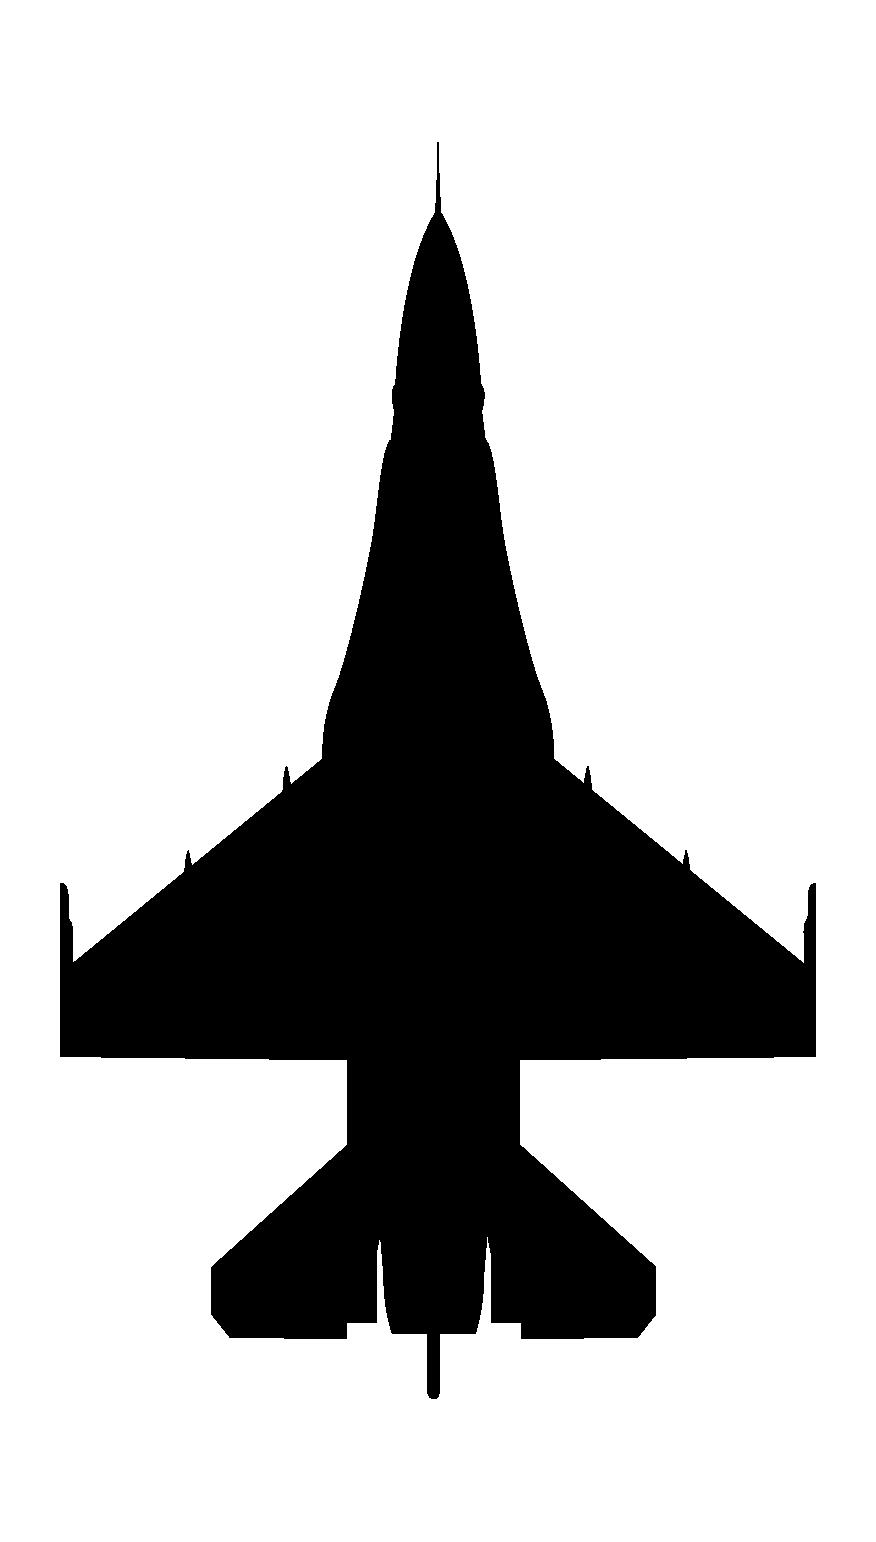
\includegraphics[
                    width=7.5mm,
                ]{diagrams/aircraft/silhouette_f16_top.pdf}
            };
    
            % BANDIT
            \draw[rounded corners, ->] 
            (0,20) -- +(90:15);
    
            % help line
            \draw[thin, dashed] 
            (0,20) -- (0,0);
    
            \draw[thin]
            (0,10) arc (-90:90:10) node[pos=0.125, below right]{\small\titlefont 110-180$^\circ$};
    
        \end{tikzpicture}
        \caption{Drag}
        \label{fig:aa_weap:bvr:ta:drag}
    \end{subfigure}
    \caption{Top down view illustrating target aspect classification}
    \label{fig:aa_weap:bvr:ta}
\end{figure}

\clearpage